\chapter{中文章節}
\label{c:template}

Attention plays an important role in human vision. For example, when
we look at an image, our eye movements comprise a succession of {\em
fixations} (repetitive positioning of eyes to parts of the image)
and {\em saccades} (rapid eye jump). Those parts of the image that
cause eye fixations and capture primary attention are called {\em
regions of interest} (ROIs). Studies in visual attention and eye
movement have shown that humans generally only attend to a few ROIs.
Detecting these visually attentive regions in images is challenging
but useful in many multimedia applications, such as automatic
thumbnail cropping, object recognition, content-based image
retrieval, adaptive image compression and automatic browsing in
small-screen devices.

Many algorithms have been proposed for automatic ROI detection in
images. Unfortunately, these methods were often evaluated only on
specific and small data sets that are not publicly available. The
lack of published {\em benchmarks} makes experiments non-repeatable
and quantitative evaluation difficult. However, as recommended by
the latest ACM SIGMM retreat, repeatable experiments using published
benchmarks are important for advancing the multimedia research
field~\cite{Rowe:2005:ASR}.

\begin{figure}
\centering
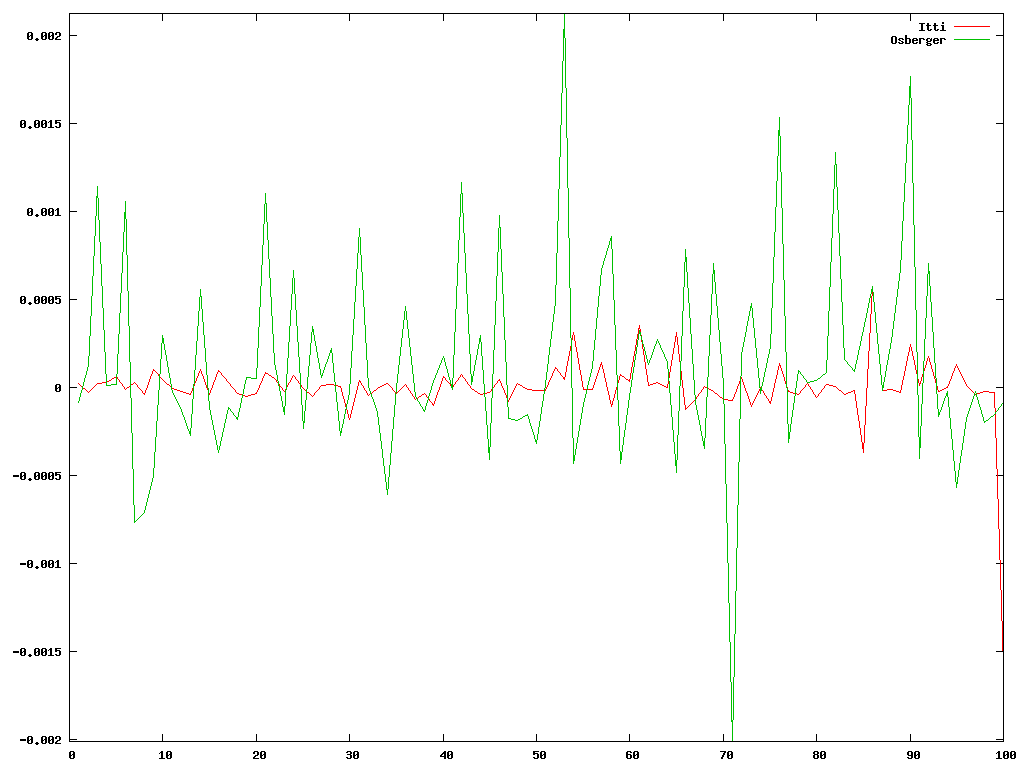
\includegraphics[width=0.45\textwidth]{sample}
\caption{kl-distance}
\label{kl}
\end{figure}

\begin{table}[t]
\begin{center}
\begin{tabular}{lcc}

\hline
                    &  {\small Itti's method}     & {\small Fuzzy growing}    \\
\hline
{\small Precision}           &  0.4475    & 0.4506 \\
{\small Recall}              &  0.5515    & 0.5542 \\
\hline

\end{tabular}
\caption[Evaluation of FOA sets]{\small Evaluation of FOA sets. } \label{t:FOA}
\end{center}
\end{table}
